Відновимо ваги зваженого графа ${ \bf C_3}$, знаючи його структуру і підспектри, тобто спектри деяких його індукованих підграфів. 

\begin{figure}[h]
    \centering
    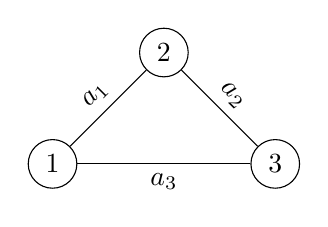
\begin{tikzpicture}[node distance={20mm}, main/.style = {draw, circle}]
    \node[main] (1) {$1$}; 
    \node[main] (2)[above right of=1] {$2$};
    \node[main] (3)[below right of=2] {$3$};
    \draw (1) -- node [midway, above, sloped] {$a_1$}(2);
    \draw (2) -- node [ above, midway, sloped] {$a_2$}(3);
    \draw (3) -- node [ below, midway, sloped] {$a_3$}(1);
    \end{tikzpicture}\\
    \caption{$\bf C_3$}
    \label{ex2:image}
\end{figure}

\begin{figure}[h]
    \centering
     \begin{subfigure}[h]{0.3\linewidth}
        \centering
        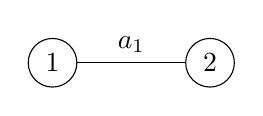
\begin{tikzpicture}[node distance={20mm}, main/.style = {draw, circle}]
            \node[main] (1) {$1$}; 
            \node[main] (2)[right of=1] {$2$};
            \draw (1) -- node [midway, above, sloped] {$a_1$}(2);
        \end{tikzpicture}\\
        \caption{}
        \label{exv1:image}
    \end{subfigure}
     \begin{subfigure}[h]{0.3\linewidth}
        \centering
        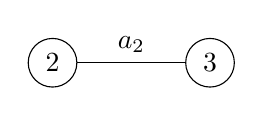
\begin{tikzpicture}[node distance={20mm}, main/.style = {draw, circle}]
            \node[main] (2){$2$};
            \node[main] (3)[right of=2] {$3$};
            \draw (2) -- node [ above, midway, sloped] {$a_2$}(3);
        \end{tikzpicture}\\
        \caption{}
        \label{exv2:image}
    \end{subfigure}
     \begin{subfigure}[h]{0.3\linewidth}
        \centering
        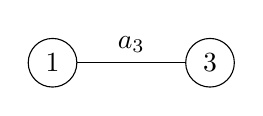
\begin{tikzpicture}[node distance={20mm}, main/.style = {draw, circle}]
            \node[main] (1) {$1$}; 
            \node[main] (3)[right of=1] {$3$};
            \draw (3) -- node [ above, midway, sloped] {$a_3$}(1);
        \end{tikzpicture}\\
        \caption{}
        \label{exv3:image}
    \end{subfigure}
    \caption{Підграфи ${\bf C_3}$}
    \label{EXv1:image}
\end{figure}

Так як для кожного власного підграфа, що є ребром, $P(\lambda)=\lambda^2-a_i^2$, то за трьома підспектрами, можна відновити ваги на ребрах графа ${\bf C_3}$, тобто $a_1,a_2,a_3$.

\textit{Чи можна відновити ваги графа ${\bf C_3}$ тільки за двома підспектрами?}\\
Для набору з двох підспектрів можна взяти спектр вихідного графа $\sigma({\bf C_3})$ і спектр графа з видаленням 1 вершини:  $\sigma({\bf C_3}-\{i\})$, де $i$ --- одна з трьох вершин.
З видаленням вершини отримаємо ребро, зі спектра якого можна відновити вагу одного ребра графа.
\begin{equation}\label{C3eq1}
P_{\bf C_3}(\lambda)=\lambda^3 - \lambda(a_1^2+a_2^2+a_3^2)-2a_1a_2a_3\end{equation}
Знаючи ліву частину характеристичного многочлена (\ref{C3eq1}) і вагу одного ребра не можна відновити однозначно ваги всього графа через симетричність.

\textit{Наприклад}, ми однозначно відновлюємо вагу $a_1$ ребра $(1,2)$ підграфа\\ ${\bf C_3}-\{3\}$ 
Тоді з характеристичного многочлена (\ref{C3eq1}) ми маємо таку систему рівнянь:
\begin{equation}\label{c3eq}
   \begin{cases}
    a_2a_3 = b\\
    a_2^2 +a_3^2= c
    \end{cases}, 
\end{equation}

де $b,\ c$ --- коефіцієнти з характеристичного многочлена, що відомі нам за умовою задачі. 

Виразимо у першому рівнянні змінну $a_2$ через змінну $a_3$($a_3 > 0)$
\[\begin{cases}
a_2 = \frac{b}{a_3}\\
(\frac{b}{a^3})^2 +a_3^2= c
\end{cases}\]
Помножимо друге рівняння на $a_3$ і знайдемо розв'язки такого біквадратного рівняння: $(\frac{b}{a_3})^2 +a_3^2= c \Rightarrow$ 
$ a_3^4 - c a_3^2 + b^2 = 0$\\
Нехай $a_3^2 = t,\ t\geq0$, отримаємо таке квадратне рівняння:
\[t^2-c t +b^2 =0\]
\[D = c^2-4b^2\]
\[t_{1,2} = \frac{c\pm\sqrt{c^2-4b^2}}{2}\]
Оскільки $t$ має бути більше або рівним нулю, то знайдемо, коли\\
$c\pm\sqrt{c^2-4b^2}\geq 0$. $c+\sqrt{c^2-4b^2}$ завжди більше 0, бо $c>0$ і $\sqrt{c^2-4b^2}\geq0$. Розглянемо, чи $c-\sqrt{c^2-4b^2}\geq 0$.
\[c\geq\sqrt{c^2-4b^2}\]
\[a_2^2 +a_3^2 \geq \sqrt{(a_2^2 +a_3^2)^2-4a_2^2a_3^2}\]
\[a_2^2 +a_3^2 \geq \sqrt{a_2^4+2a_2^2a_3^2 +a_3^4-4a_2^2a_3^2}\]
\[a_2^2 +a_3^2 \geq \sqrt{(a_2^2 - a_3^2)^2}\]
\[a_2^2 +a_3^2 \geq a_2^2 - a_3^2\]
\[a_2^2 +a_3^2 \geq a_2^2 - a_3^2\]
\[2a_3^2 \geq 0\]
Отже, ми отримали що $c-\sqrt{c^2-4b^2}$ також завжди більше нуля.
\[a_3 = \pm \sqrt{t}\]
Оскільки ваги графа є додатніми, то $a_3 =  \sqrt{\frac{c+\sqrt{c^2-4b^2}}{2}}$ і $a_2 = \sqrt{\frac{2}{c+\sqrt{c^2-4b^2}}}b$ або $a_3 =  \sqrt{\frac{c-\sqrt{c^2-4b^2}}{2}}$ і $a_2 = \sqrt{\frac{2}{c-\sqrt{c^2-4b^2}}}b$.

Аналогічно, якщо виразити у першому рівнянні системи (\ref{c3eq}) змінну $a_3$ через змінну $a_2$($a_2 > 0$). Отримаємо біквадратне рівняння: $ a_2^4 - c a_2^2 + b^2 = 0$ і такі самі результати.

 З цієї системи рівнянь отримуємо симетричні розв'язки: $a_3 =  \sqrt{\frac{c+\sqrt{c^2-4b^2}}{2}}$ і $a_2 = \sqrt{\frac{2}{c+\sqrt{c^2-4b^2}}}b$ або $a_3 =  \sqrt{\frac{c-\sqrt{c^2-4b^2}}{2}}$ і $a_2 = \sqrt{\frac{2}{c-\sqrt{c^2-4b^2}}}b$. Оскільки нам важлива нумерація вершин, то нам не достатньо знати $2$ підспектрів для відновлення ваг зваженого графа $\bf C_3$.
 
\textit{ Отже, $Srn(C_3) = 3$.}